% !TEX root = main.tex
\section{順運動学と逆運動学}

\subsection{運動方程式}

リンク1を手で基準位置から回転させてリンク1の基準位置からの回転角 $\theta_x(t)$ がさほど大きくなければ、リンク4は静止したままである。
したがって、$P_1$, $P_5$ の角度 $\theta_x(t)$, $\theta_y(t)$ がその基準角度の近傍で動作するとすると、リンク1とリンク4との干渉は無視できる(実際、リンク1あるいはリンク4を手で微小回転させてもリンク4あるいはリンク1は静止したままである)。
このとき、リンク1、リンク4の運動方程式は
\begin{equation}
\begin{aligned}
    J_x \ddot{\theta}_x(t) &= -c_x \dot{\theta}_x(t) + \tau_x(t) \\
    J_y \ddot{\theta}_y(t) &= -c_y \dot{\theta}_y(t) + \tau_y(t)
\end{aligned}
\label{eq:2.1}
\end{equation}
となる。
ただし、$\tau_x(t)$, $\tau_y(t)$ は軸 $P_1$, $P_5$ に加わるトルク、$J_x$, $J_y$ はリンク1、リンク4の慣性モーメントであり、$c_x$, $c_y$ は軸 $P_1$, $P_5$ の粘性摩擦係数である。
また、モータドライバに加える電圧 $v_x(t)$, $v_y(t)$ とトルク $\tau_x(t)$, $\tau_y(t)$ が比例関係
\begin{equation}
\left\{
\begin{aligned}
\tau_x(t) &= k_{fx} v_x(t) \\
\tau_y(t) &= k_{fy} v_y(t)
\end{aligned}
\right.
\label{eq:2.2}
\end{equation}
にあると仮定すると、

\begin{equation}
\begin{aligned}
    J_x \ddot{\theta}_x(t) &= -c_x \dot{\theta}_x(t) + k_{fx} v_x(t) \\
    J_y \ddot{\theta}_y(t) &= -c_y \dot{\theta}_y(t) + k_{fy} v_y(t)
\end{aligned}
\label{eq:2.3}
\end{equation}
であるから、$v_x(t)$, $v_y(t)$ から $\theta_x(t)$, $\theta_y(t)$ への伝達関数 $G_x(s)$, $G_y(s)$ は

\begin{equation}
\left\{
\begin{aligned}
G_x(s) &= \frac{b_x}{s(s+a_x)}, \quad a_x = \frac{c_x}{J_x}, \quad b_x = \frac{k_{fx}}{J_x} \\
G_y(s) &= \frac{b_y}{s(s+a_y)}, \quad a_y = \frac{c_y}{J_y}, \quad b_y = \frac{k_{fy}}{J_y}
\end{aligned}
\right.
\label{eq:2.4}
\end{equation}
となる。

\subsection{逆運動学}

ここでは,手先にあたる軸 $P_3$ の座標 $(x, y)$ からモータの回転軸 $P_1$, $P_5$ の角度 $\theta_x$, $\theta_y$ を求める.このように,手先の座標から回転角を求めることを逆運動学という.

\begin{figure}[H]
  \centering
  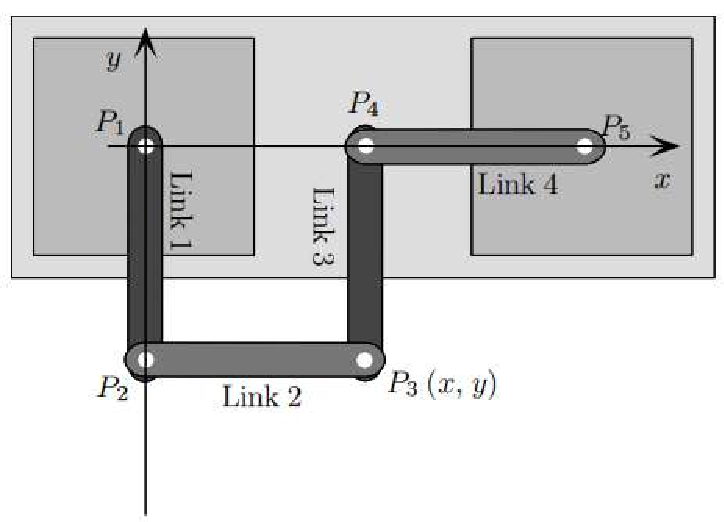
\includegraphics[width=0.65\textwidth]{figure/robot_fig3.pdf} % ←図2.1のファイル名に合わせて変更
  \caption{初期位置(基準位置)}
  \label{fig:init_pos}
\end{figure}

\begin{figure}[H]
  \centering
  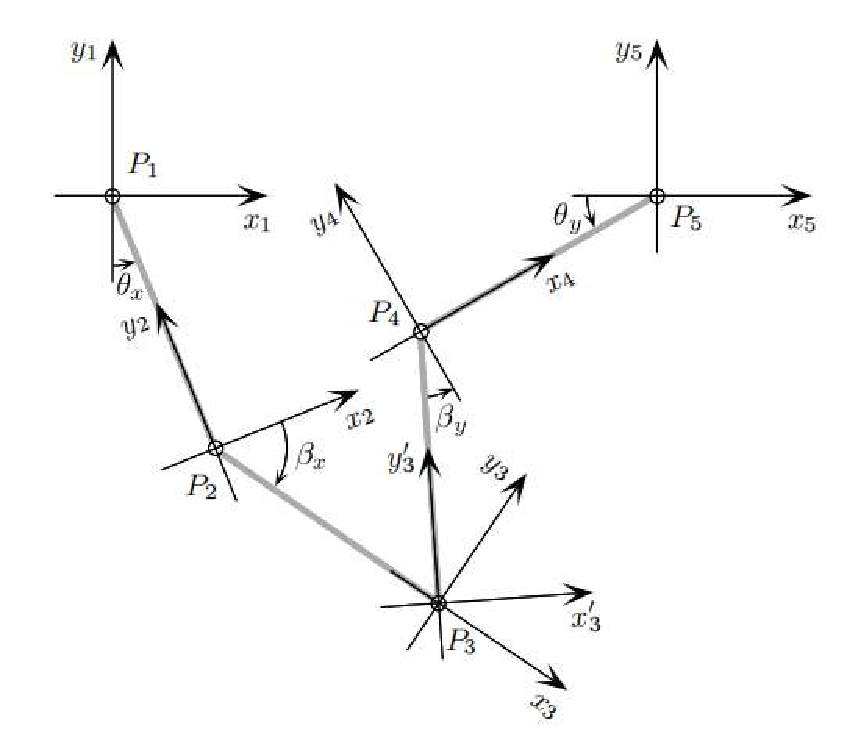
\includegraphics[width=0.65\textwidth]{figure/robot_fig4.pdf} % ←図2.2のファイル名に合わせて変更
  \caption{逆運動学のための各座標系}
  \label{fig:frames}
\end{figure}

図~\ref{fig:frames} に示すように,リンク1,リンク2に関しては $x_1 y_1$ 座標系と $x_2 y_2$ 座標系,$x_2 y_2$ 座標系と $x_3 y_3$ 座標系は

\begin{align}
    \begin{bmatrix}
    x_1 \\ y_1
    \end{bmatrix}
    &=
    \begin{bmatrix}
    \cos\theta_x & -\sin\theta_x \\
    \sin\theta_x & \cos\theta_x
    \end{bmatrix}
    \begin{bmatrix}
    x_2 \\ y_2
    \end{bmatrix}
    +
    \begin{bmatrix}
    \ell \sin\theta_x \\ -\ell \cos\theta_x
    \end{bmatrix}
    \tag{2.5} \\
    %
    \begin{bmatrix}
    x_2 \\ y_2
    \end{bmatrix}
    &=
    \begin{bmatrix}
    \cos(-\beta_x) & -\sin(-\beta_x) \\
    \sin(-\beta_x) & \cos(-\beta_x)
    \end{bmatrix}
    \begin{bmatrix}
    x_3 \\ y_3
    \end{bmatrix}
    +
    \begin{bmatrix}
    \ell \cos\beta_x \\ -\ell \sin\beta_x
    \end{bmatrix} \notag \\
    &=
    \begin{bmatrix}
    \cos\beta_x & \sin\beta_x \\
    -\sin\beta_x & \cos\beta_x
    \end{bmatrix}
    \begin{bmatrix}
    x_3 \\ y_3
    \end{bmatrix}
    +
    \begin{bmatrix}
    \ell \cos\beta_x \\ -\ell \sin\beta_x
    \end{bmatrix}
    \tag{2.6}
    \end{align}
    

という関係にある.(2.5),(2.6) 式を書き換えると,

\begin{align}
    \begin{bmatrix}
    x_1 & y_1 & 1
    \end{bmatrix}^T
    &= T_{12}
    \begin{bmatrix}
    x_2 & y_2 & 1
    \end{bmatrix}^T
    \tag{2.7} \\
    \begin{bmatrix}
    x_2 & y_2 & 1
    \end{bmatrix}^T
    &= T_{23}
    \begin{bmatrix}
    x_3 & y_3 & 1
    \end{bmatrix}^T
    \tag{2.8}
    \end{align}
    
    \[
    T_{12} =
    \begin{bmatrix}
    \cos\theta_x & -\sin\theta_x & \ell \sin\theta_x \\
    \sin\theta_x & \cos\theta_x & -\ell \cos\theta_x \\
    0 & 0 & 1
    \end{bmatrix},
    \quad
    T_{23} =
    \begin{bmatrix}
    \cos\beta_x & \sin\beta_x & -\ell \sin\beta_x \\
    -\sin\beta_x & \cos\beta_x & \ell \cos\beta_x \\
    0 & 0 & 1
    \end{bmatrix}
    \]
    

となるから,$x_1 y_1$ 座標系と $x_3 y_3$ 座標系との間に以下の関係式が成立する.

\begin{align}
\begin{bmatrix}
x_1 & y_1 & 1
\end{bmatrix}^T
=
T_{13}
\begin{bmatrix}
x_3 & y_3 & 1
\end{bmatrix}^T,
\quad
T_{13} = T_{12} T_{23}
\tag{2.9}
\end{align}

(2.9) 式を利用して,$x_3 y_3$ 座標系の原点 $P_3$ を $x_1 y_1$ 座標系で表すと,

\begin{align}
    \begin{bmatrix}
    x & y & 1
    \end{bmatrix}^T
    &= T_{13}
    \begin{bmatrix}
    0 & 0 & 1
    \end{bmatrix}^T \notag \\
    &=
    \left[
    \ell \cos\theta_x \cos\beta_x + \ell \sin\theta_x \sin\beta_x + \ell \sin\theta_x,
    \quad
    -\ell \cos\theta_x \sin\beta_x + \ell \sin\theta_x \cos\beta_x - \ell \cos\theta_x,
    \quad
    1
    \right]^T \notag \\
    &=
    \left[
    \ell \cos(\theta_x - \beta_x) + \ell \sin\theta_x,
    \quad
    \ell \sin(\theta_x - \beta_x) - \ell \cos\theta_x,
    \quad
    1
    \right]^T
    \tag{2.10}
    \end{align}
    
となる.(2.10) 式より

\begin{align}
    \left\{
    \begin{aligned}
    x &= \ell \cos(\theta_x - \beta_x) + \ell \sin\theta_x \\
    y &= \ell \sin(\theta_x - \beta_x) - \ell \cos\theta_x
    \end{aligned}
    \right.
    \tag{2.11}
    \end{align}
    
    \begin{align}
    &\Longrightarrow
    \left\{
    \begin{aligned}
    x - \ell \sin\theta_x &= \ell \cos(\theta_x - \beta_x) \\
    y + \ell \cos\theta_x &= \ell \sin(\theta_x - \beta_x)
    \end{aligned}
    \right. \notag \\
    &\Longrightarrow
    (x - \ell \sin\theta_x)^2 + (y + \ell \cos\theta_x)^2 = \ell^2
    \tag{2.12}
    \end{align}
    
    
    
    であるから,$P_3$ は中心 $(\ell \sin\theta_x, -\ell \cos\theta_x)$,半径 $\ell$ の円上を移動することがわかる.
    (2.12)式を書き換えると
    
    \begin{align}
    x^2 + y^2 - 2\ell (\sin\theta_x x - \cos\theta_x y) = 0
    \notag
    \end{align}
    
    \[
    \Longrightarrow
    \quad
    x^2 + y^2 - 2\ell \sqrt{x^2 + y^2} \sin(\theta_x + \phi_x) = 0
    \quad , \quad
    \left\{
    \begin{aligned}
    \cos\phi_x &= \frac{x}{\sqrt{x^2 + y^2}} \\
    \sin\phi_x &= \frac{y}{\sqrt{x^2 + y^2}}
    \end{aligned}
    \right.
    \]
    
    \[
    \Longrightarrow
    \quad
    \sin(\theta_x + \phi_x) = \frac{\sqrt{x^2 + y^2}}{2\ell}
    \quad , \quad
    \theta_x = \sin^{-1} \left( \frac{\sqrt{x^2 + y^2}}{2\ell} \right) - \phi_x
    \tag{2.13}
    \]
    
    となる.したがって,$P_3$ の座標 $(x, y)$ からモータの回転軸 $P_1$ の角度 $\theta_x$ が次式により求まる.
    
    \begin{align}
    \theta_x = \sin^{-1} \left( \frac{\sqrt{x^2 + y^2}}{2\ell} \right) + \tan^{-1} \left( \frac{y}{x} \right)
    \tag{2.14}
    \end{align}
    
    同様に,リンク3,リンク4に関して考えると,$x_1 y_1$ 座標系と $x_5 y_5$ 座標系,$x_5 y_5$ 座標系と $x_4 y_4$ 座標系,$x_4 y_4$ 座標系と $x_3' y_3'$ 座標系は

    \begin{align}
    \begin{bmatrix}
    x_1 \\
    y_1
    \end{bmatrix}
    &=
    \begin{bmatrix}
    1 & 0 \\
    0 & 1
    \end{bmatrix}
    \begin{bmatrix}
    x_5 \\
    y_5
    \end{bmatrix}
    +
    \begin{bmatrix}
    2\ell \\
    0
    \end{bmatrix}
    \tag{2.15} \\
    \begin{bmatrix}
    x_5 \\
    y_5
    \end{bmatrix}
    &=
    \begin{bmatrix}
    \cos\theta_y & -\sin\theta_y \\
    \sin\theta_y & \cos\theta_y
    \end{bmatrix}
    \begin{bmatrix}
    x_4 \\
    y_4
    \end{bmatrix}
    +
    \begin{bmatrix}
    -\ell \cos\theta_y \\
    -\ell \sin\theta_y
    \end{bmatrix}
    \tag{2.16} \\
    \begin{bmatrix}
    x_4 \\
    y_4
    \end{bmatrix}
    &=
    \begin{bmatrix}
    \cos(-\beta_y) & -\sin(-\beta_y) \\
    \sin(-\beta_y) & \cos(-\beta_y)
    \end{bmatrix}
    \begin{bmatrix}
    x_3' \\
    y_3'
    \end{bmatrix}
    +
    \begin{bmatrix}
    -\ell \sin\beta_y \\
    -\ell \cos\beta_y
    \end{bmatrix} \notag \\
    &=
    \begin{bmatrix}
    \cos\beta_y & \sin\beta_y \\
    -\sin\beta_y & \cos\beta_y
    \end{bmatrix}
    \begin{bmatrix}
    x_3' \\
    y_3'
    \end{bmatrix}
    +
    \begin{bmatrix}
    -\ell \sin\beta_y \\
    -\ell \cos\beta_y
    \end{bmatrix}
    \tag{2.17}
    \end{align}
    
    という関係にある.(2.15),(2.16),(2.17) 式を書き換えると,
    
    \begin{align}
    \begin{bmatrix}
    x_1 & y_1 & 1
    \end{bmatrix}^T
    &= T_{15}
    \begin{bmatrix}
    x_5 & y_5 & 1
    \end{bmatrix}^T
    \tag{2.18} \\
    \begin{bmatrix}
    x_5 & y_5 & 1
    \end{bmatrix}^T
    &= T_{54}
    \begin{bmatrix}
    x_4 & y_4 & 1
    \end{bmatrix}^T
    \tag{2.19} \\
    \begin{bmatrix}
    x_4 & y_4 & 1
    \end{bmatrix}^T
    &= T_{43}'
    \begin{bmatrix}
    x_3' & y_3' & 1
    \end{bmatrix}^T
    \tag{2.20}
    \end{align}
    
    ここで各変換行列は
    
    \[
    T_{15} =
    \begin{bmatrix}
    1 & 0 & 2\ell \\
    0 & 1 & 0 \\
    0 & 0 & 1
    \end{bmatrix}
    \quad
    T_{54} =
    \begin{bmatrix}
    \cos\theta_y & -\sin\theta_y & -\ell \cos\theta_y \\
    \sin\theta_y & \cos\theta_y  & -\ell \sin\theta_y \\
    0 & 0 & 1
    \end{bmatrix}
    \quad
    T_{43}' =
    \begin{bmatrix}
    \cos\beta_y & \sin\beta_y & -\ell \sin\beta_y \\
    -\sin\beta_y & \cos\beta_y & -\ell \cos\beta_y \\
    0 & 0 & 1
    \end{bmatrix}
    \]
    
    となるから,$x_1 y_1$ 座標系と $x_3' y_3'$ 座標系との間に以下の関係式が成立する.
    
    \begin{align}
    \begin{bmatrix}
    x_1 & y_1 & 1
    \end{bmatrix}^T
    = T'_{13}
    \begin{bmatrix}
    x_3' & y_3' & 1
    \end{bmatrix}^T
    ,
    \quad
    T'_{13} = T_{15} T_{54} T'_{43}
    \tag{2.21}
    \end{align}

    (2.21) 式を利用して,$x'_3 y'_3$ 座標系の原点 $P_3$ を $x_1 y_1$ 座標系で表すと,

    \begin{align}
        \begin{bmatrix}
        x & y & 1
        \end{bmatrix}^T
        &= T'_{13}
        \begin{bmatrix}
        0 \\ 0 \\ 1
        \end{bmatrix}
        \notag \\
        &=
        \left[
        \begin{array}{c}
        -\ell \cos\theta_y \sin\beta_y + \ell \sin\theta_y \cos\beta_y - \ell \cos\theta_y + 2\ell \\
        -\ell \cos\theta_y \cos\beta_y + \ell \sin\theta_y \sin\beta_y - \ell \sin\theta_y \\
        1
        \end{array}
        \right]
        \notag \\
        &=
        \left[
        \begin{array}{c}
        -\ell \cos(\theta_y + \beta_y) - \ell \cos\theta_y + 2\ell \\
        -\ell \sin(\theta_y + \beta_y) - \ell \sin\theta_y \\
        1
        \end{array}
        \right]
        \tag{2.22}
        \end{align}
        
    
    となる.(2.22) 式より
    
    \begin{align}
    \left\{
    \begin{aligned}
    x' &= x - 2\ell = -\ell \cos(\theta_y + \beta_y) - \ell \cos\theta_y \\
    y &= -\ell \sin(\theta_y + \beta_y) - \ell \sin\theta_y
    \end{aligned}
    \right.
    \tag{2.23}
    \end{align}
    
    \begin{align}
    \Longrightarrow
    \left\{
    \begin{aligned}
    x' + \ell \cos\theta_y &= -\ell \cos(\theta_y + \beta_y) \\
    y + \ell \sin\theta_y &= -\ell \sin(\theta_y + \beta_y)
    \end{aligned}
    \right.
    \Longrightarrow
    (x' + \ell \cos\theta_y)^2 + (y + \ell \sin\theta_y)^2 = \ell^2
    \tag{2.24}
    \end{align}
    
    であるから,$P_3$ は中心 $(2\ell - \ell \cos\theta_y,\ -\ell \sin\theta_y)$,半径 $\ell$ の円上を移動することがわかる.(2.24) 式を書き換えると
    
    \begin{align}
        x'^2 + y^2 + 2\ell (x'\cos\theta_y + y\sin\theta_y) = 0 \notag \\
        \Longrightarrow \quad
        x'^2 + y^2 - 2\ell \sqrt{x'^2 + y^2} \sin(\theta_y + \phi_y) = 0,
        \quad
        \left\{
        \begin{aligned}
        \cos\phi_y &= -\dfrac{y}{\sqrt{x'^2 + y^2}} \\
        \sin\phi_y &= -\dfrac{x'}{\sqrt{x'^2 + y^2}}
        \end{aligned}
        \right.
        \notag \\
        \Longrightarrow \quad
        \sin(\theta_y + \phi_y) = \dfrac{\sqrt{x'^2 + y^2}}{2\ell} \notag \\
        \Longrightarrow \quad
        \theta_y = \sin^{-1}\left( \dfrac{\sqrt{x'^2 + y^2}}{2\ell} \right) - \phi_y
        \tag{2.25}
        \end{align}
        
    
    したがって,$P_3$ の座標 $(x, y)$ からモータの回転軸 $P_5$ の角度 $\theta_y$ が次式により求まる.
    
    \begin{align}
    \theta_y
    = \sin^{-1} \left( \dfrac{\sqrt{x'^2 + y^2}}{2\ell} \right)
    - \tan^{-1} \left( \dfrac{x'}{y} \right) \notag \\
    = \sin^{-1} \left( \dfrac{\sqrt{(x - 2\ell)^2 + y^2}}{2\ell} \right)
    - \tan^{-1} \left( \dfrac{x - 2\ell}{y} \right)
    \tag{2.26}
    \end{align}
    

    \subsection{順運動学}

    ここでは、モータの回転軸 $P_1$,$P_5$ の角度 $\theta_x$,$\theta_y$ から手先 $P_3$ の座標 $(x, y)$ を求める。
    このように、回転軸から手先の座標を求めることを順運動学という。
    
    \par
    軸 $P_2$,$P_4$ の回転角 $\beta_x$,$\beta_y$ が検出可能であれば (2.11) 式や (2.23) 式により手先 $P_3$ の座標 $(x, y)$ を求めることができるが、本実験装置は軸 $P_2$,$P_4$ にはセンサが取り付けられていない。
    そこで、$x_1 y_1$ 座標系、$x_2 y_2$ 座標系、$x_3 y_3$ 座標系を考える代わりに、図 \ref{fig:kinematics1} に示す
    $x_1 y_1$ 座標系、$x_2 y_2$ 座標系、$x_m y_m$ 座標系、$x'_3 y'_3$ 座標系を考える。
    
    \begin{figure}[H]
        \centering
        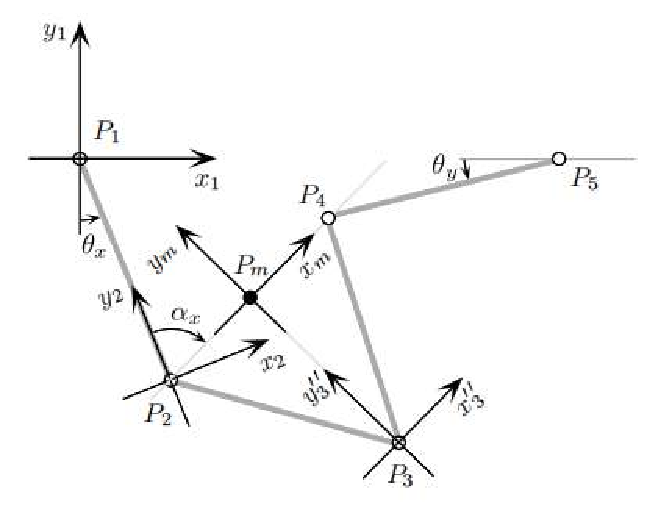
\includegraphics[width=0.8\textwidth]{figure/robot_fig5.pdf} 
        \caption{順運動学のための各座標系1}
        \label{fig:kinematics1}
    \end{figure}
    
    \begin{figure}[H]
        \centering
        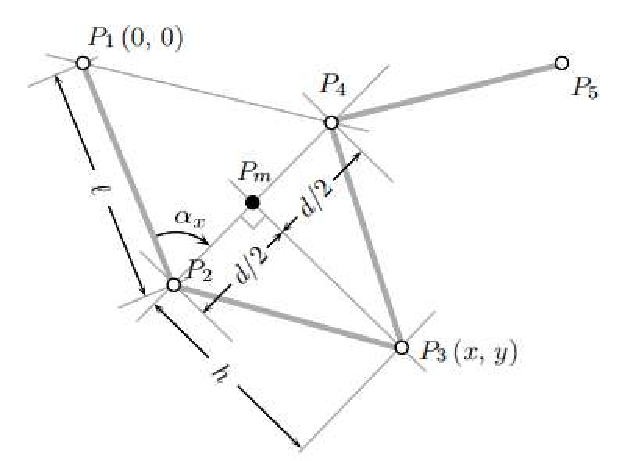
\includegraphics[width=0.8\textwidth]{figure/robot_fig6.pdf}
        \caption{順運動学のための各座標系2}
        \label{fig:kinematics2}
    \end{figure}
    
図 \ref{fig:kinematics1},\ref{fig:kinematics2} より
$x_2 y_2$ 座標系と $x_m y_m$ 座標系,
$x_m y_m$ 座標系と $x'_3 y'_3$ 座標系は

\begin{align}
\begin{bmatrix}
x_2 \\
y_2
\end{bmatrix}
&=
\begin{bmatrix}
\cos\left( \dfrac{\pi}{2} - \alpha_x \right) & -\sin\left( \dfrac{\pi}{2} - \alpha_x \right) \\
\sin\left( \dfrac{\pi}{2} - \alpha_x \right) & \cos\left( \dfrac{\pi}{2} - \alpha_x \right)
\end{bmatrix}
\begin{bmatrix}
x_m \\
y_m
\end{bmatrix}
+
\begin{bmatrix}
\dfrac{d}{2}\cos\left( \dfrac{\pi}{2} - \alpha_x \right) \\
\dfrac{d}{2}\sin\left( \dfrac{\pi}{2} - \alpha_x \right)
\end{bmatrix} \notag \\
&=
\begin{bmatrix}
\sin\alpha_x & -\cos\alpha_x \\
\cos\alpha_x & \sin\alpha_x
\end{bmatrix}
\begin{bmatrix}
x_m \\
y_m
\end{bmatrix}
+
\begin{bmatrix}
\dfrac{d}{2}\sin\alpha_x \\
\dfrac{d}{2}\cos\alpha_x
\end{bmatrix}
\tag{2.27}
\end{align}
\begin{align}
    \begin{bmatrix}
    x_m \\ y_m
    \end{bmatrix}
    &=
    \begin{bmatrix}
    1 & 0 \\
    0 & 1
    \end{bmatrix}
    \begin{bmatrix}
    x''_3 \\ y''_3
    \end{bmatrix}
    +
    \begin{bmatrix}
    0 \\ -h
    \end{bmatrix}
    \tag{2.28}
    \end{align}
    
    という関係にある.(2.27),(2.28) 式を書き換えると,

    \begin{align}
        \begin{bmatrix}
        x_2 & y_2 & 1
        \end{bmatrix}^T
        &= T_{2m}
        \begin{bmatrix}
        x_m & y_m & 1
        \end{bmatrix}^T
        \tag{2.29}
        \\
        \begin{bmatrix}
        x_m & y_m & 1
        \end{bmatrix}^T
        &= T''_{m3}
        \begin{bmatrix}
        x''_3 & y''_3 & 1
        \end{bmatrix}^T
        \tag{2.30}
        \end{align}
        
        \[
        T_{2m} =
        \begin{bmatrix}
        \sin\alpha_x & -\cos\alpha_x & \dfrac{d}{2}\sin\alpha_x \\
        \cos\alpha_x & \sin\alpha_x & \dfrac{d}{2}\cos\alpha_x \\
        0 & 0 & 1
        \end{bmatrix}
        ,\quad
        T''_{m3} =
        \begin{bmatrix}
        1 & 0 & 0 \\
        0 & 1 & -h \\
        0 & 0 & 1
        \end{bmatrix}
        \]
        となるから,$x_1 y_1$ 座標系と $x''_3 y''_3$ 座標系との間に以下の関係式が成立する.

        \[
        \begin{bmatrix}
        x_1 & y_1 & 1
        \end{bmatrix}^T
        =
        T''_{13}
        \begin{bmatrix}
        x''_3 & y''_3 & 1
        \end{bmatrix}^T
        ,\quad
        T''_{13} = T_{12} T_{2m} T''_{m3}
        \tag{2.31}
        \]
        
        (2.31) 式を利用して,$x''_3 y''_3$ 座標系の原点 $P_3$ を $x_1 y_1$ 座標系で表すと,
        
\[
\begin{aligned}
\begin{bmatrix}
x & y & 1
\end{bmatrix}^T
&=
T''_{13}
\begin{bmatrix}
0 & 0 & 1
\end{bmatrix}^T \\[2ex]
&=
\left[
\begin{array}{c}
h(\cos\theta_x\cos\alpha_x + \sin\theta_x\sin\alpha_x) - \dfrac{d}{2}(\sin\theta_x\cos\alpha_x - \cos\theta_x\sin\alpha_x) + \ell\sin\theta_x \\
h(\sin\theta_x\cos\alpha_x - \cos\theta_x\sin\alpha_x) + \dfrac{d}{2}(\cos\theta_x\cos\alpha_x + \sin\theta_x\sin\alpha_x) - \ell\cos\theta_x \\
1
\end{array}
\right] \\[2ex]
&=
\left[
\begin{array}{c}
h\cos(\theta_x-\alpha_x) - \dfrac{d}{2}\sin(\theta_x-\alpha_x) + \ell\sin\theta_x \\
h\sin(\theta_x-\alpha_x) + \dfrac{d}{2}\cos(\theta_x-\alpha_x) - \ell\cos\theta_x \\
1
\end{array}
\right]
\end{aligned}
\tag{2.32}
\]

となる.したがって,$d$,$h$,$\alpha_x$ が求まれば手先 $P_3$ の座標が
\[
\left\{
\begin{aligned}
x &= h \cos(\theta_x - \alpha_x) - \dfrac{d}{2} \sin(\theta_x - \alpha_x) + \ell \sin\theta_x \\
y &= h \sin(\theta_x - \alpha_x) + \dfrac{d}{2} \cos(\theta_x - \alpha_x) - \ell \cos\theta_x
\end{aligned}
\right.
\tag{2.33}
\]

により求まる.

$x_1 y_1$ 座標系における $P_2$,$P_4$ の座標をそれぞれ $(p_{2x}, p_{2y})$,$(p_{4x}, p_{4y})$ とすると,

\[
\left\{
\begin{aligned}
p_{2x} &= \ell \sin\theta_x \\
p_{2y} &= -\ell \cos\theta_x
\end{aligned}
\right.
,\quad
\left\{
\begin{aligned}
p_{4x} &= 2\ell - \ell \cos\theta_y \\
p_{4y} &= -\ell \sin\theta_y
\end{aligned}
\right.
\tag{2.34}
\]

であるから,$d$ は

\[
d = P_2P_4 = \sqrt{(p_{2x} - p_{4x})^2 + (p_{2y} - p_{4y})^2}
\tag{2.35}
\]

と定まる.

また,$h$ は三角形 $P_m P_2 P_3$ における三平方の定理より

\[
h = \sqrt{\ell^2 - \left( \dfrac{d}{2} \right)^2}
\tag{2.36}
\]

と定まり,$\alpha_x$ は三角形 $P_1 P_2 P_4$ における余弦定理より

\[
(P_1P_4)^2 = \ell^2 + d^2 - 2d\ell \cos\alpha_x
\]
\[
\quad \Rightarrow \quad
p_{4x}^2 + p_{4y}^2 = \ell^2 + d^2 - 2d\ell \cos\alpha_x
\]
\[
\quad \Rightarrow \quad
\alpha_x = \cos^{-1} \left( \dfrac{\ell^2 + d^2 - (p_{4x}^2 + p_{4y}^2)}{2d\ell} \right)
\tag{2.37}
\]

と定まる.

        